% Twiin Pitch Deck — 12 slides, 16:9 · Onest font
% Compile: ./compile-pitch.sh

\documentclass[aspectratio=169,11pt]{beamer}

\usepackage{fontspec}
\usepackage{xcolor}
\usepackage{graphicx}
\usepackage{tikz}
\usepackage{hyperref}
\usepackage{etoolbox}

\usetikzlibrary{positioning,arrows.meta,shapes.geometric,calc,fit,backgrounds}

%%% Onest (matches frontend) %%%
\setsansfont{Onest}[
    Path=fonts/,
    Extension=.ttf,
    UprightFont=Onest,
    BoldFont=Onest,
    UprightFeatures={Weight=400},
    BoldFeatures={Weight=700},
    Scale=0.97,
]
\setmainfont{Onest}[
    Path=fonts/,
    Extension=.ttf,
    UprightFont=Onest,
    BoldFont=Onest,
    UprightFeatures={Weight=400},
    BoldFeatures={Weight=700},
    Scale=0.97,
]
\newfontfamily\OnestBold{Onest}[
    Path=fonts/,
    Extension=.ttf,
    UprightFont=Onest,
    Weight=700,
    Scale=0.97,
]

%%% Brand tokens (from app.css) %%%
\definecolor{primary}{HTML}{163300}
\definecolor{accent}{HTML}{9FE870}
\definecolor{charcoal}{HTML}{1A1A1A}
\definecolor{foreground}{HTML}{0F0F0F}
\definecolor{ghost}{HTML}{F8FCF5}
\definecolor{card}{HTML}{FCFEFB}
\definecolor{border}{HTML}{E8F0E4}
\definecolor{muted}{HTML}{5A5A5A}
\definecolor{mutedfg}{HTML}{8A8A8A}

%%% TikZ palette %%%
\definecolor{nodegreen}{HTML}{e8f9d4}
\definecolor{nodeblue}{HTML}{FCFEFB}
\definecolor{nodeyellow}{HTML}{f0f7e8}
\definecolor{nodepink}{HTML}{f5f5f5}
\definecolor{bordergreen}{HTML}{9FE870}
\definecolor{borderblue}{HTML}{163300}
\definecolor{borderyellow}{HTML}{c8e6a0}
\definecolor{borderlight}{HTML}{E8F0E4}

\tikzset{
    flowstep/.style={
        draw=borderlight, fill=card, line width=0.6pt,
        minimum width=2.5cm, minimum height=0.75cm,
        font=\scriptsize, align=center
    },
    flowstepwide/.style={
        draw=borderlight, fill=card, line width=0.6pt,
        minimum width=8.8cm, minimum height=0.68cm,
        font=\scriptsize, align=center
    },
    flowstephi/.style={
        draw=bordergreen, fill=nodegreen, line width=1pt,
        minimum width=2.5cm, minimum height=0.75cm,
        font=\scriptsize\bfseries, align=center
    },
    userbox/.style={
        draw=bordergreen, fill=nodegreen, line width=0.8pt,
        minimum width=2.8cm, minimum height=0.82cm,
        font=\scriptsize, align=center
    },
    appbox/.style={
        draw=borderlight, fill=card, line width=0.6pt,
        minimum width=3cm, minimum height=0.82cm,
        font=\scriptsize, align=center
    },
    servicebox/.style={
        draw=borderyellow, fill=nodeyellow, line width=0.6pt,
        minimum width=3cm, minimum height=0.82cm,
        font=\scriptsize, align=center
    },
    chainbox/.style={
        draw=borderlight, fill=ghost, line width=0.6pt,
        minimum width=3cm, minimum height=0.82cm,
        font=\scriptsize, align=center
    },
    decision/.style={
        draw=borderyellow, fill=nodeyellow, diamond, line width=0.6pt,
        inner sep=1.5pt, aspect=2.2,
        font=\scriptsize, align=center
    },
    arrow/.style={-{Latex[length=2mm]}, semithick, color=mutedfg},
}

%%% UI helpers %%%
\newcommand{\twiincard}[2]{%
    \begin{tikzpicture}
        \node[
            draw=border, fill=card, line width=0.6pt,
            inner sep=10pt, text width=#1, align=left
        ] {#2};
    \end{tikzpicture}%
}

\newcommand{\statcard}[2]{%
    \begin{tikzpicture}
        \node[
            draw=border, fill=card, line width=0.6pt,
            minimum width=3.35cm, minimum height=1.35cm,
            inner sep=6pt, align=left
        ] {%
            {\fontsize{20}{22}\selectfont\bfseries\color{primary} #1}\\[2pt]
            {\footnotesize\color{muted} #2}%
        };
    \end{tikzpicture}%
}

\newcommand{\callout}[1]{%
    \begin{tikzpicture}
        \node[
            draw=border, fill=nodegreen, line width=0.6pt,
            inner sep=10pt, text width=0.88\textwidth, align=center
        ] {{\color{primary}\bfseries #1}};
    \end{tikzpicture}%
}

\newcommand{\tagpill}[1]{%
    {\footnotesize\bfseries\color{primary}%
    \tikz[baseline=(t.base)]{
        \node[fill=accent, inner xsep=8pt, inner ysep=3pt] (t) {#1};
    }}%
}

%%% Beamer theme %%%
\usetheme{default}
\usecolortheme{default}
\usefonttheme{professionalfonts}

\setbeamercolor{normal text}{fg=foreground,bg=ghost}
\setbeamercolor{structure}{fg=primary}
\setbeamercolor{frametitle}{fg=primary,bg=ghost}
\setbeamercolor{footline}{fg=muted,bg=ghost}

\setbeamertemplate{navigation symbols}{}

\setbeamertemplate{itemize item}{%
    \textcolor{primary}{\raisebox{0.12ex}{\rule{0.35em}{0.35em}}}%
}
\setbeamertemplate{itemize enitemize item}{%
    \textcolor{accent}{\raisebox{0.1ex}{\rule{0.25em}{0.25em}}}%
}

\setbeamersize{text margin left=1.1cm, text margin right=1.1cm}

\setbeamertemplate{background}{%
    \begin{tikzpicture}[remember picture,overlay]
        \fill[ghost] (current page.south west) rectangle (current page.north east);
        \fill[primary] ([yshift=-2.5pt]current page.north west) rectangle (current page.north east);
    \end{tikzpicture}%
}

\setbeamerfont{frametitle}{size=\Large, series=\bfseries}
\setbeamerfont{framesubtitle}{size=\normalsize, series=\bfseries}

\setbeamertemplate{frametitle}{%
    \vspace{0.55em}
    {\OnestBold\usebeamerfont{frametitle}\color{primary}\insertframetitle\par}%
    \vspace{0.35em}%
}

\setbeamertemplate{footline}{%
    \leavevmode%
    \begin{tikzpicture}[remember picture,overlay]
        \fill[card] ([yshift=2.4ex]current page.south west) rectangle (current page.south east);
        \draw[border, line width=0.4pt] ([yshift=2.4ex]current page.south west) -- (current page.south east);
        \fill[accent] ([yshift=2.4ex]current page.south west) rectangle
            ([xshift={0.1\paperwidth},yshift=2.4ex]current page.south west);
        \node[anchor=south west, xshift=1.1em, yshift=0.55em] at (current page.south west) {%
            \footnotesize\color{muted}Twiin · Somnia Agentathon 2026%
        };
        \node[anchor=south east, xshift=-1.1em, yshift=0.55em] at (current page.south east) {%
            \footnotesize\color{muted}\insertframenumber\,/\inserttotalframenumber%
        };
    \end{tikzpicture}%
    \vskip0pt%
}

\hypersetup{
    colorlinks=true,
    linkcolor=primary,
    urlcolor=primary,
    pdfauthor={Team Twiin},
    pdftitle={Twiin Pitch Deck},
}

\title{Twiin}
\subtitle{Own the AI Agent}
\author{Team Twiin}
\date{Somnia Agentathon 2026}

\begin{document}

% ── 1 · Title ───────────────────────────────────────────────
{
\setbeamertemplate{background}{%
    \begin{tikzpicture}[remember picture,overlay]
        \fill[ghost] (current page.south west) rectangle (current page.north east);
        \fill[primary] (current page.north west) rectangle ([yshift=-4pt]current page.north east);
        \fill[accent] ([yshift=-4pt]current page.north west) rectangle ([yshift=-7pt]current page.north east);
    \end{tikzpicture}%
}
\begin{frame}[plain]
    \begin{center}
        \vspace{0.15cm}
        \tagpill{Somnia Agentathon 2026}\\[0.7cm]
        
\includegraphics[width=0.5\textwidth]{twiin-banner.png}\\[0.55cm]
        {\LARGE\bfseries\color{primary} Own the AI Agent}\\[0.4cm]
        \twiincard{0.72\textwidth}{%
            {\normalsize\color{muted}%
            Mint an NFT with its own wallet.\;
            Approve a plan once.\;
            Keepers execute every step on-chain.}%
        }\\[0.7cm]
        {\footnotesize\color{mutedfg}
            \href{https://twiin-frontend.vercel.app/}{\texttt{twiin-frontend.vercel.app}}%
        }
    \end{center}
\end{frame}
}

% ── 2 · Problem ─────────────────────────────────────────────
\begin{frame}{The Problem}
    \vspace{-0.2cm}
    \begin{columns}[T,onlytextwidth]
        \begin{column}{0.32\textwidth}
            \centering\twiincard{2.9cm}{%
                \textbf{\color{primary}Centralized}\\[4pt]
                {\footnotesize Agents run on servers you don't control}%
            }
        \end{column}
        \begin{column}{0.32\textwidth}
            \centering\twiincard{2.9cm}{%
                \textbf{\color{primary}No ownership}\\[4pt]
                {\footnotesize No on-chain limits or verifiable execution}%
            }
        \end{column}
        \begin{column}{0.32\textwidth}
            \centering\twiincard{2.9cm}{%
                \textbf{\color{primary}Manual ops}\\[4pt]
                {\footnotesize Babysit infra, click every step}%
            }
        \end{column}
    \end{columns}
    \vspace{0.65cm}
    \centering\callout{You rent the agent. You don't own it.}
\end{frame}

% ── 3 · Solution ────────────────────────────────────────────
\begin{frame}{The Solution}
    \begin{columns}[T,onlytextwidth]
        \begin{column}{0.58\textwidth}
            \begin{itemize}\setlength\itemsep{0.55em}
                \item \textbf{ERC-721 NFT} owns an \textbf{ERC-6551 wallet} on Somnia
                \item Fund once, set caps, \textbf{approve one plan}
                \item Keepers + validators dispatch, rate, and pay on-chain
                \item No user-operated server. No cron jobs.
            \end{itemize}
        \end{column}
        \begin{column}{0.38\textwidth}
            \centering
            \twiincard{3.4cm}{%
                {\footnotesize\color{muted}One signature}\\[6pt]
                {\Large\bfseries\color{primary}1×}\\[4pt]
                {\footnotesize\color{muted}The agent runs itself}%
            }
        \end{column}
    \end{columns}
\end{frame}

% ── 4 · How It Works ────────────────────────────────────────
\begin{frame}{How It Works}
    \centering
    \vspace{0.15cm}
    \resizebox{0.92\textwidth}{!}{%
    
\begin{tikzpicture}[
        node distance=0cm and 0.55cm,
        every node/.style={font=\footnotesize, align=center},
    ]
        \node[flowstep, minimum width=2.35cm, minimum height=1.05cm] (s1) {Connect\\Wallet};
        \node[flowstep, minimum width=2.35cm, minimum height=1.05cm, right=of s1] (s2) {Deploy\\Agent};
        \node[flowstep, minimum width=2.35cm, minimum height=1.05cm, right=of s2] (s3) {Plan\\Goal};
        \node[flowstephi, minimum width=2.35cm, minimum height=1.05cm, right=of s3] (s4) {Approve\\Once};
        \node[flowstep, minimum width=2.35cm, minimum height=1.05cm, right=of s4] (s5) {Watch\\Live};
        \draw[arrow] (s1) -- (s2);
        \draw[arrow] (s2) -- (s3);
        \draw[arrow] (s3) -- (s4);
        \draw[arrow] (s4) -- (s5);
        \node[below=0.18cm of s4, font=\tiny\bfseries, color=primary] {only signature};
    \end{tikzpicture}%
  }
    \vspace{0.65cm}
    \callout{Approve Once is the only MetaMask popup in the entire demo}
\end{frame}

% ── 5 · Somnia Native Agentation ────────────────────────────
\begin{frame}{Somnia Native Agentation}
    \vspace{-0.15cm}
    \begin{columns}[T,onlytextwidth]
        \begin{column}{0.52\textwidth}
            \begin{itemize}\setlength\itemsep{0.4em}
                \item Native steps route through the \textbf{Somnia Agents API}
                \item Orchestrator calls \texttt{createRequest} with ABI-encoded payloads
                \item \textbf{3-validator subcommittee} reaches consensus on-chain
                \item \texttt{StepConsensusReached} — verifiable validator receipts
                \item Relay keeper bridges results back to \texttt{AgentOrchestrator}
            \end{itemize}
        \end{column}
        \begin{column}{0.46\textwidth}
            \centering
            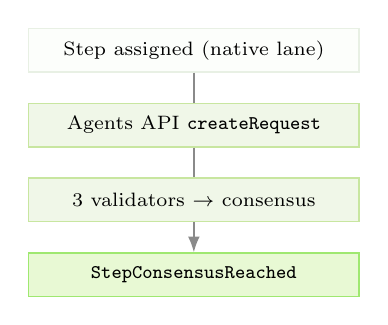
\begin{tikzpicture}[node distance=0.38cm, every node/.style={font=\tiny, align=center}]
                \node[flowstepwide, minimum width=4.2cm, minimum height=0.55cm] (s1) {Step assigned (native lane)};
                \node[flowstepwide, minimum width=4.2cm, minimum height=0.55cm, below=of s1, fill=nodeyellow, draw=borderyellow] (s2) {Agents API \texttt{createRequest}};
                \node[flowstepwide, minimum width=4.2cm, minimum height=0.55cm, below=of s2, fill=nodeyellow, draw=borderyellow] (s3) {3 validators $\rightarrow$ consensus};
                \node[flowstepwide, minimum width=4.2cm, minimum height=0.55cm, below=of s3, fill=nodegreen, draw=bordergreen] (s4) {\texttt{StepConsensusReached}};
                \draw[arrow] (s1) -- (s2) -- (s3) -- (s4);
            \end{tikzpicture}
        \end{column}
    \end{columns}
    \vspace{0.35cm}
    {\footnotesize\color{muted}
        Native catalog (configIds 0–5):
        \textbf{janice} · \textbf{web-intel} · \textbf{somnia-oracle} · \textbf{analysis-bot} · \textbf{reporter-bot} · \textbf{executor-bot}%
    }
\end{frame}

% ── 6 · Somnia Primitives ───────────────────────────────────
\begin{frame}{Somnia Primitives in Twiin}
    \vspace{-0.1cm}
    \begin{columns}[T,onlytextwidth]
        \begin{column}{0.32\textwidth}
            \centering\twiincard{2.85cm}{%
                \textbf{\color{primary}ERC-6551}\\[4pt]
                {\footnotesize NFT owns a token-bound account — the agent's on-chain wallet. One \texttt{deployTwiin} tx mints, funds, and seeds policy.}%
            }
        \end{column}
        \begin{column}{0.32\textwidth}
            \centering\twiincard{2.85cm}{%
                \textbf{\color{primary}Agents API}\\[4pt]
                {\footnotesize Native lane dispatches to Somnia base agents via on-chain requests. Validator consensus — not a centralized cron.}%
            }
        \end{column}
        \begin{column}{0.32\textwidth}
            \centering\twiincard{2.85cm}{%
                \textbf{\color{primary}Reactivity}\\[4pt]
                {\footnotesize \texttt{subscribePull} + \texttt{pullForRefresh} on the 6551 account. Chain-side oracle refresh without off-chain schedulers.}%
            }
        \end{column}
    \end{columns}
    \vspace{0.5cm}
    \centering\callout{Built for Somnia Shannon testnet · chainId 50312 · STT gas}
\end{frame}

% ── 7 · Architecture ────────────────────────────────────────
\begin{frame}{System Architecture}
    \centering\vspace{-0.15cm}
    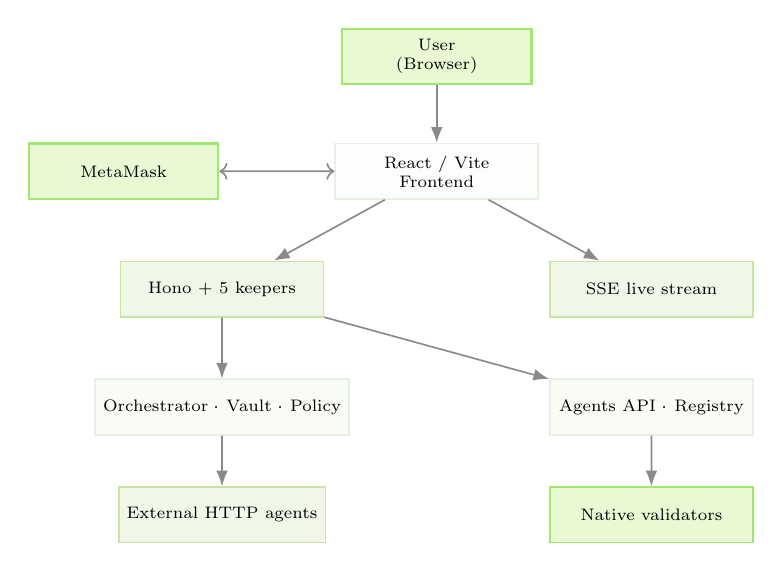
\begin{tikzpicture}[
        node distance=0.65cm and 0.85cm,
        every node/.style={font=\scriptsize, align=center},
        scale=0.86, transform shape,
    ]
        \node[userbox] (user) {User\\(Browser)};
        \node[appbox, below=0.85cm of user] (frontend) {React / Vite\\Frontend};
        \node[userbox, left=1.7cm of frontend] (wallet) {MetaMask};
        \node[servicebox, below left=0.9cm and 0.15cm of frontend] (backend) {Hono + 5 keepers};
        \node[servicebox, below right=0.9cm and 0.15cm of frontend] (sse) {SSE live stream};
        \node[chainbox, below=0.9cm of backend] (contracts) {Orchestrator · Vault · Policy};
        \node[chainbox, below=0.9cm of sse] (agents) {Agents API · Registry};
        \node[servicebox, below=0.75cm of agents, fill=nodegreen, draw=bordergreen] (native) {Native validators};
        \node[servicebox, below=0.75cm of contracts] (http) {External HTTP agents};
        \draw[arrow] (user) -- (frontend);
        \draw[arrow, <->] (wallet) -- (frontend);
        \draw[arrow] (frontend) -- (backend);
        \draw[arrow] (frontend) -- (sse);
        \draw[arrow] (backend) -- (contracts);
        \draw[arrow] (backend) -- (agents);
        \draw[arrow] (agents) -- (native);
        \draw[arrow] (contracts) -- (http);
    \end{tikzpicture}
\end{frame}

% ── 8 · Task Lifecycle ──────────────────────────────────────
\begin{frame}{Task Lifecycle}
    \centering\vspace{-0.1cm}
    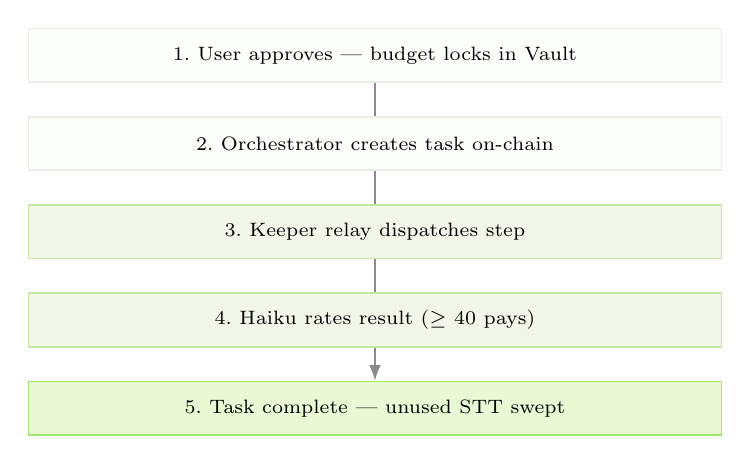
\begin{tikzpicture}[node distance=0.42cm, every node/.style={font=\scriptsize, align=center}]
        \node[flowstepwide] (s1) {1.\ User approves — budget locks in Vault};
        \node[flowstepwide, below=of s1] (s2) {2.\ Orchestrator creates task on-chain};
        \node[flowstepwide, below=of s2, fill=nodeyellow, draw=borderyellow] (s3) {3.\ Keeper relay dispatches step};
        \node[flowstepwide, below=of s3, fill=nodeyellow, draw=borderyellow] (s4) {4.\ Haiku rates result ($\geq$ 40 pays)};
        \node[flowstepwide, below=of s4, fill=nodegreen, draw=bordergreen] (s5) {5.\ Task complete — unused STT swept};
        \draw[arrow] (s1) -- (s2) -- (s3) -- (s4) -- (s5);
    \end{tikzpicture}
\end{frame}

% ── 9 · Two-Lane Registry ─────────────────────────────────────
\begin{frame}{Two-Lane Registry}
    \centering
    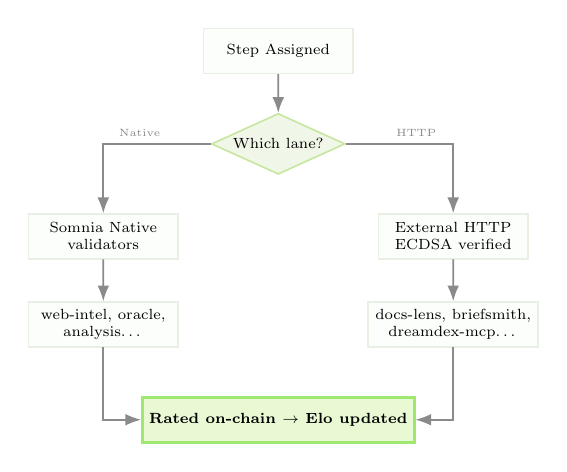
\begin{tikzpicture}[
        node distance=0.5cm and 0.9cm,
        every node/.style={font=\scriptsize, align=center},
        scale=0.76, transform shape,
    ]
        \node[flowstep] (assigned) {Step Assigned};
        \node[decision, below=0.65cm of assigned] (lane) {Which lane?};
        \node[flowstep, below left=0.9cm and 1.1cm of lane] (native) {Somnia Native\\validators};
        \node[flowstep, below right=0.9cm and 1.1cm of lane] (external) {External HTTP\\ECDSA verified};
        \node[flowstep, below=0.7cm of native] (nagents) {web-intel, oracle,\\analysis\ldots};
        \node[flowstep, below=0.7cm of external] (eagents) {docs-lens, briefsmith,\\dreamdex-mcp\ldots};
        \node[flowstephi, below=1.6cm of lane, yshift=-2.1cm] (rated) {Rated on-chain $\rightarrow$ Elo updated};
        \draw[arrow] (assigned) -- (lane);
        \draw[arrow] (lane) -| node[pos=0.2, font=\tiny, above left] {Native} (native);
        \draw[arrow] (lane) -| node[pos=0.2, font=\tiny, above right] {HTTP} (external);
        \draw[arrow] (native) -- (nagents);
        \draw[arrow] (external) -- (eagents);
        \draw[arrow] (nagents) |- (rated);
        \draw[arrow] (eagents) |- (rated);
    \end{tikzpicture}
\end{frame}

% ── 10 · Demo Pipeline ──────────────────────────────────────
\begin{frame}{Live Demo Pipeline}
    \centering
    \tagpill{Goal: How healthy is the Somnia ecosystem?}\\[0.35cm]
    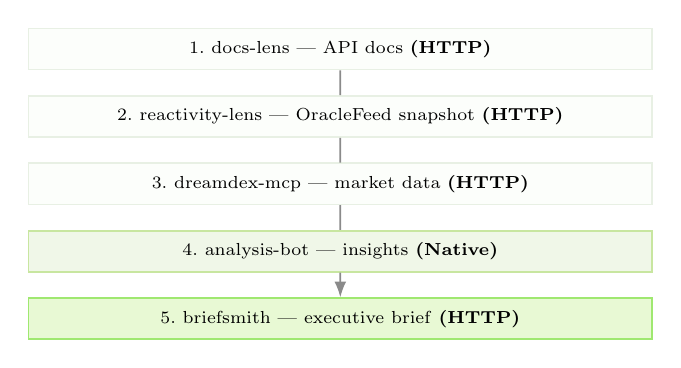
\begin{tikzpicture}[node distance=0.35cm, every node/.style={font=\scriptsize, align=center}, scale=0.9, transform shape]
        \node[flowstepwide, minimum height=0.58cm] (s1) {1.\ docs-lens — API docs \textbf{(HTTP)}};
        \node[flowstepwide, minimum height=0.58cm, below=of s1] (s2) {2.\ reactivity-lens — OracleFeed snapshot \textbf{(HTTP)}};
        \node[flowstepwide, minimum height=0.58cm, below=of s2] (s3) {3.\ dreamdex-mcp — market data \textbf{(HTTP)}};
        \node[flowstepwide, minimum height=0.58cm, below=of s3, fill=nodeyellow, draw=borderyellow] (s4) {4.\ analysis-bot — insights \textbf{(Native)}};
        \node[flowstepwide, minimum height=0.58cm, below=of s4, fill=nodegreen, draw=bordergreen] (s5) {5.\ briefsmith — executive brief \textbf{(HTTP)}};
        \draw[arrow] (s1) -- (s2) -- (s3) -- (s4) -- (s5);
    \end{tikzpicture}
    \vspace{0.35cm}
    \callout{One signature starts the entire pipeline}
\end{frame}

% ── 11 · Built & Shipped ───────────────────────────────────────
\begin{frame}{Built \& Shipped}
    \vspace{-0.25cm}
    \begin{columns}[c,onlytextwidth]
        \begin{column}{0.24\textwidth}\centering\statcard{94+}{Contract tests}\end{column}
        \begin{column}{0.24\textwidth}\centering\statcard{6}{Native agents}\end{column}
        \begin{column}{0.24\textwidth}\centering\statcard{5}{Keeper bots}\end{column}
        \begin{column}{0.24\textwidth}\centering\statcard{7}{External agents}\end{column}
    \end{columns}
    \vspace{0.4cm}
    \begin{columns}[T,onlytextwidth]
        \begin{column}{0.48\textwidth}
            \textbf{\color{primary}Full stack}
            \begin{itemize}\setlength\itemsep{0.3em}
                \item 11 Solidity contracts on Somnia
                \item React console + marketplace UI
                \item Claude Haiku planner \& rater
            \end{itemize}
        \end{column}
        \begin{column}{0.48\textwidth}
            \textbf{\color{primary}Live}
            \begin{itemize}\setlength\itemsep{0.3em}
                \item \href{https://twiin-frontend.vercel.app/}{twiin-frontend.vercel.app}
                \item \href{https://github.com/wurli-sh/twiin}{github.com/wurli-sh/twiin}
                \item Somnia Shannon · chainId \textbf{50312}
            \end{itemize}
        \end{column}
    \end{columns}
\end{frame}

% ── 12 · Thank You ──────────────────────────────────────────
{
\setbeamertemplate{background}{%
    \begin{tikzpicture}[remember picture,overlay]
        \fill[primary] (current page.south west) rectangle (current page.north east);
    \end{tikzpicture}%
}
\begin{frame}[plain]
    \begin{center}
        \vspace{1.1cm}
        {\fontsize{28}{32}\selectfont\bfseries\color{accent} Thank You}\\[0.75cm]
        {\Large\color{ghost} Deploy an agent. Approve once.\\
        The chain does the rest.}\\[1.1cm]
        {\normalsize\color{accent}
            \href{https://github.com/wurli-sh/twiin}{\texttt{github.com/wurli-sh/twiin}}\\[0.25cm]
            \href{https://twiin-frontend.vercel.app/}{\texttt{twiin-frontend.vercel.app}}\\[0.35cm]
            {\color{ghost!80}Team Twiin · Somnia Agentathon 2026}%
        }
    \end{center}
\end{frame}
}

\end{document}
